\documentclass[]{article}
\usepackage{lmodern}
\usepackage{amssymb,amsmath}
\usepackage{ifxetex,ifluatex}
\usepackage{fixltx2e} % provides \textsubscript
\ifnum 0\ifxetex 1\fi\ifluatex 1\fi=0 % if pdftex
  \usepackage[T1]{fontenc}
  \usepackage[utf8]{inputenc}
\else % if luatex or xelatex
  \ifxetex
    \usepackage{mathspec}
  \else
    \usepackage{fontspec}
  \fi
  \defaultfontfeatures{Ligatures=TeX,Scale=MatchLowercase}
  \newcommand{\euro}{€}
\fi
% use upquote if available, for straight quotes in verbatim environments
\IfFileExists{upquote.sty}{\usepackage{upquote}}{}
% use microtype if available
\IfFileExists{microtype.sty}{%
\usepackage{microtype}
\UseMicrotypeSet[protrusion]{basicmath} % disable protrusion for tt fonts
}{}
\usepackage[margin=1in]{geometry}
\usepackage{hyperref}
\PassOptionsToPackage{usenames,dvipsnames}{color} % color is loaded by hyperref
\hypersetup{unicode=true,
            pdftitle={Wait\ldots{} random isn't randomf},
            pdfauthor={Mike},
            pdfborder={0 0 0},
            breaklinks=true}
\urlstyle{same}  % don't use monospace font for urls
\usepackage{graphicx,grffile}
\makeatletter
\def\maxwidth{\ifdim\Gin@nat@width>\linewidth\linewidth\else\Gin@nat@width\fi}
\def\maxheight{\ifdim\Gin@nat@height>\textheight\textheight\else\Gin@nat@height\fi}
\makeatother
% Scale images if necessary, so that they will not overflow the page
% margins by default, and it is still possible to overwrite the defaults
% using explicit options in \includegraphics[width, height, ...]{}
\setkeys{Gin}{width=\maxwidth,height=\maxheight,keepaspectratio}
\setlength{\parindent}{0pt}
\setlength{\parskip}{6pt plus 2pt minus 1pt}
\setlength{\emergencystretch}{3em}  % prevent overfull lines
\providecommand{\tightlist}{%
  \setlength{\itemsep}{0pt}\setlength{\parskip}{0pt}}
\setcounter{secnumdepth}{0}

%%% Use protect on footnotes to avoid problems with footnotes in titles
\let\rmarkdownfootnote\footnote%
\def\footnote{\protect\rmarkdownfootnote}

%%% Change title format to be more compact
\usepackage{titling}

% Create subtitle command for use in maketitle
\newcommand{\subtitle}[1]{
  \posttitle{
    \begin{center}\large#1\end{center}
    }
}

\setlength{\droptitle}{-2em}
  \title{Wait\ldots{} random isn't randomf}
  \pretitle{\vspace{\droptitle}\centering\huge}
  \posttitle{\par}
  \author{Mike}
  \preauthor{\centering\large\emph}
  \postauthor{\par}
  \predate{\centering\large\emph}
  \postdate{\par}
  \date{2018-04-18}


% Redefines (sub)paragraphs to behave more like sections
\ifx\paragraph\undefined\else
\let\oldparagraph\paragraph
\renewcommand{\paragraph}[1]{\oldparagraph{#1}\mbox{}}
\fi
\ifx\subparagraph\undefined\else
\let\oldsubparagraph\subparagraph
\renewcommand{\subparagraph}[1]{\oldsubparagraph{#1}\mbox{}}
\fi


\begin{document}
\maketitle

Here's a nice little mind blower: it's actually incredibly hard to find
and measure something that is truly random. This is actually a bit of a
problem as there's so many places where random numbers are needed, in
this blog post I'll use a few running examples where random number
generation is needed:

\begin{enumerate}
\def\labelenumi{\arabic{enumi}.}
\tightlist
\item
  The gambling sector, pretty much everywhere from shuffling cards in
  online poker (and in casinos for the particularly high tech ones) to
  slot machines for obvious reasons.
\item
  Simulation, when it's not deterministic you need random numbers.
  Similarly, video games can be seen as big simulations and generally
  require random numbers.
\item
  Random assignment, making sure that everything is fair when say
  assigning placebos in a clinical trial.
\end{enumerate}

\subsection{Motivation}\label{motivation}

It seems like it shouldn't be a problem, like everything seems random so
it shouldn't be too hard to just get a random number. This is true,
there're loads of approaches which you can take to obtain random numbers
such as:

\begin{itemize}
\tightlist
\item
  Measuring radioactivity, place a radioactive isotope in front of a
  device called a Geiger counter, observing the time between clicks is
  random. PRO: The numbers are truly random CONS: Health issues of
  sitting near a radioactive isotope every time you need a random
  number.
\item
  Observing human behaviour, people are random, if you observe things
  like extremely small movements of a mouse or time between keystrokes
  to the microsecond can be used. PRO: Can get massive amounts of random
  numbers if you have a database of people willing to supply their
  keystrokes. CON: Good luck getting even one person to agree to giving
  you open access to their computer, you'll need thousands to get the
  amount of random numbers most applications need.
\end{itemize}

Both of these methods are highly limited in speed and require a lot of
legwork to get up and running. \#\# Pseudorandom numbers So, how do we
actually get these random numbers quickly? You'll notice that nearly
every programming language has a command to generate random numbers for
example runif in R, this all done with a method called pseudorandom
number generation, it generates sequences of numbers which look random
but in fact they're not. These numbers are completely determined by a
mathematical formula which is designed to produce sequences of random
looking numbers.

Fact is that for applications like simulation and video games we really
don't care as long as they look random which makes. Take applications
like security and gambling, if these numbers are in any way predictable
then there's a massive problem with random number generation. Take an
online slot machine, if someone figured out the underlying random number
generator then they could just bet small when they know they're not
going to win; then, when a winning spin is coming up they just put a big
bet on. Therefore, if gambling companies go for pseudorandom numbers
they should really ensure that it's virtually impossible to reverse
engineer.

\subsection{Example generator -- Linear congruential
generator}\label{example-generator-linear-congruential-generator}

Here I'll give an example of one of the earliest pseudorandom number
generator. It's defined as follows \[X_n=(aX_{n-1}+c)mod m\]

so you have to specify * a the multiplier * m the modulus * c the
increment * \(X_0\) a value to start the algorithm

In this generator, the next value is completely determined by the value
that came before it. I find this quite mind blowing as it's one of the
most commonly used random number generators. It creates sequences that
look very random. Aditionally you can use some fancy mathematical proofs
that gaurentee that no two random numbers will be repeated within a
sequence of \(m\) numbers. So if you set m to be massive like \(2^{32}\)
this can make very long sequences of unique numbers.

Generators like this are good for Random assignment and simulation as
they give us billions of numbers which statistically indistiguisibly for
truely random numbers (if we choose the right formula and numbers). I'll
now show you one problem with such a generator. \#\# Cryptographically
secure pseudorandom number generator

Cryptographically secure basicly means you can give someone as many
numbers as they like and they'll never be able to reverse engineer the
generator. This is exactly what is needed for applications to gambling
and security. The linear congruential generator above does not satisfy
this property take the numbers:

\begin{quote}
5, 1, 3, 2, 6, 4, 5, 1
\end{quote}

You can easily find that a linear congruential generator with the values
c=0, a=3, m=7 generates this. Sadly even when you pick larger numbers
the same is true the formula can be reverse engineered; Therefore, more
advanced formula are required. Algorithms that have this secure property
are significantly harder to find.

\subsection{Conclusion}\label{conclusion}

\begin{figure}[htbp]
\centering
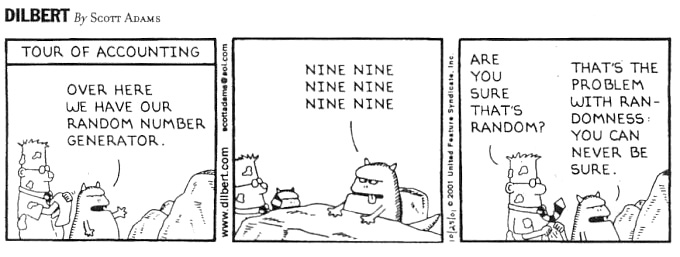
\includegraphics{../../post/img/dilbert.jpg}
\caption{Problem with random number generators.}
\end{figure}

\end{document}
